\documentclass{article}
\usepackage{amsfonts}
\usepackage[a4paper]{geometry}
\usepackage{alltt}
\usepackage{lmodern}
\usepackage{amssymb}
\usepackage{mathtools}
\usepackage{amsmath}
\usepackage{enumerate}
\usepackage{array}
\usepackage{listings}
\usepackage{fullpage}
\usepackage[parfill]{parskip}
\usepackage[utf8]{inputenc}
\usepackage[ngerman]{babel} 
\usepackage{graphicx}
\usepackage{tikz}
\usepackage{fancyhdr}
\usepackage{pgfplots}
\usepackage{multicol}

\usetikzlibrary{calc,patterns,arrows,positioning,calc,fit,shapes}

\title{GDB Uebung 2, Gruppe 61}
\author{Arne Beer, MN 6489196\\
        Oliver Heidmann, MN 6420331,
        Minh Nguyen, MN 6423136}

\begin{document}
    \maketitle
    \begin{enumerate}
        \item   \begin{enumerate}
                        \item $ $ \\ 
                            \begin{figure}[ht!]
                                \centering
                                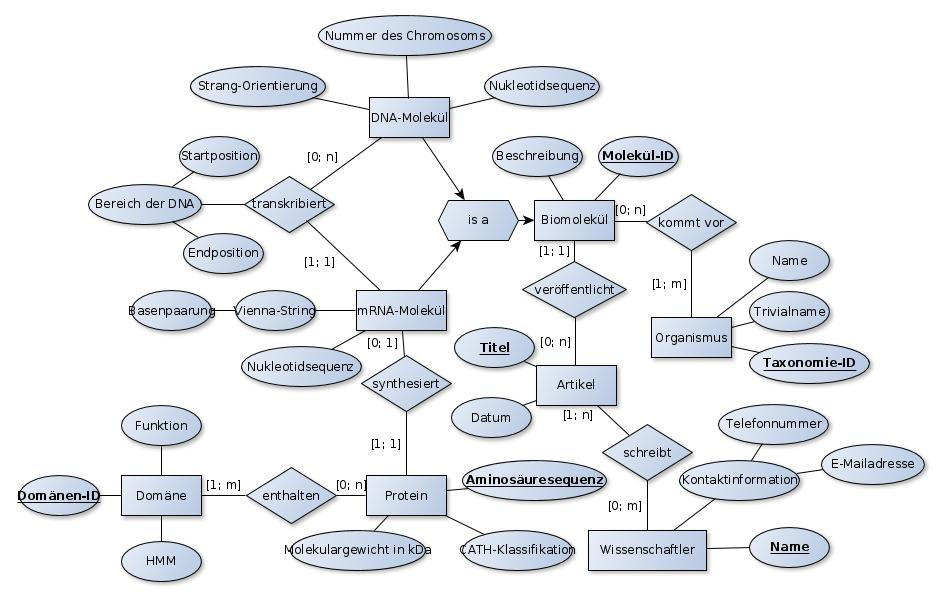
\includegraphics[width=180mm]{GDB_BLatt3_Auf1.jpg}
                                \caption{ER-Model}
                                \label{overflow}
                            \end{figure}
                \end{enumerate} 
                \newpage
        \item
                \begin{itemize}
                    \item Charakter (CID, Name, Charakterbeschreibung)
                    \item Film (Titel, Zusammenfassung, 1. Drehtag, letzter Drehtag,
                    \item Regieführung $\leftarrow$ Regisseur.Name)
                    \item Genre (Name)
                \end{itemize}
                (Partitionierungs-Modell)
                \begin{itemize}
                    \item Person (Name, DOB, Geschlecht)\\         
                    \item Regisseur (Name, Präferenz $\leftarrow$ Genre.Name)
                    \item Schauspieler (Name)
                    \item Markenzeichen (Name $\leftarrow$ Schauspieler.Name , Besonderheit)
                    \item spielt CID $\leftarrow$ Charakter.CID, Titel $\leftarrow$ Film.Titel, Name $\leftarrow$ Schauspieler.Name, Drehbeginn, Drehende, Gage)
                    \item gehört zu (Titel $\leftarrow$ Film.Titel, Name $\leftarrow$ Genre.Name)
                \end{itemize}
            \item
                \begin{enumerate}
                    \item 
                        \begin{enumerate}
                            \item Nachnamen der Rennfahrer die im Malaysia GP den ersten Platz belegt haben. {(Vettel)}
                            \item Vor- und Nachnamen der Rennfahrer, dessen Rennstall ein Budget von über 350 haben. {(Sebastian, Vettel)}
                            \item Namen der Rennställe, die im Australien GP eine Platzierung haben. {(Red Bull), (Ferrari), (McLAren)}
                        \end{enumerate}

                    \item
                        \begin{enumerate}
                            \item $\pi_{\text{Rennstall.Name}}$ ($\delta_{\text{Geburt $<$ 1984-12-31}}$ (Rennfahrer $\bowtie$ Rennstall)) \{(Red Bull), (McLaren)\}

                            \item $\pi_{\text{Vorname, Nachname, Geburt}}$ ($\pi_{\text{RID}}$ ($\delta_{\text{Name = ''Australien GP''}}$ (Rennort) $\bowtie$ Platzierung) $\bowtie \delta_{\text{Rennstall.Name = ''McLaren''}}$ (Rennfahrer $\bowtie_{\text{ RSID = Rennstall Rennstall}}$)) \{(Jenson, Button, 1980-01-19)\}


                            \item $\delta_{\text{Rennstall.Name = ''McLaren''}}$  (Rennfahrer $\bowtie_{\text{RSID = Rennstall}}$ Rennstall)) \{(Jenson, Button, 1980-01-19)\}

                            \item $\pi_{\text{Vorname, Nachname}}$ ($\delta_{\text{Nachname /= Button}}$(Rennfahrer $\bowtie_{\text{ RSID = Rennstall}}$ $\pi_{\text{RSID}}$($\delta_{\text{Nachname = Button}}$ (Rennfahrer) $\bowtie_{\text{ RSID = Rennstall}}$ Rennstall))) \{(Lewis, Hamilton)\}
                        \end{enumerate}
                    \item 
                        \begin{enumerate}
                            \item $ $
                            \begin{lstlisting}[language=SQL]
SELECT fahrer.Vorname, fahrer.Nachname, fahrer.Geburt
FROM Platzierung platz,
Rennort ort,
Rennfahrer fahrer
WHERE platz.OID = ort.OID
AND platz.RID = fahrer.RID
AND ort.Name = 'Australien GP'
AND fahrer.Rennstall = 31
                            \end{lstlisting}
                        \item $ $
                            \begin{lstlisting}[language=SQL]
SELECT Vorname, Nachname
FROM Rennfahrer
WHERE Rennstall = 31
AND Nachname <> 'Button'
                            \end{lstlisting}
                    \end{enumerate}
                \end{enumerate}
            \item 
                \begin{enumerate}
                        \item[a)] \quad \\
                        \begin{tikzpicture}[style={sibling distance=4cm}]
                    \node{\(\pi_{\text{Wohnort}}(\sigma_{\text{Name=''ChinaGP''}}(\sigma_{\text{Platz}<11}
                                ((\text{Rennfahrer $\bowtie$ Platzierung})\bowtie \text{Rennort})))\)}
                            child{node{\(\pi_{\text{Wohnort}}\)}
                                    child{node{\(\sigma_{\text{Name = ''ChinaGP''}}\)}
                                            child{node{\(\sigma_{\text{Platz}< 11}\)}
                                                    child{node{\(\text{Rennfahrer $\bowtie$ Platzierung}\)}
                                                            child{node{Rennfahrer}}
                                                            child{node{Platzierung}}
                                                    }
                                                    child{node{Rennort}
                                                    }
                                            }
                                    }
                            }
                    ;
                                
                        \end{tikzpicture} \\
                        \item[b)]\quad \\
                        \begin{tikzpicture}[style = {level distance=1.5cm},
                                            level 3/.style={sibling distance=4cm, level distance=2cm},
                                            level 4/.style={level distance=1.5cm}]
                                            
                                \node{\(\pi_{\text{Wohnort}}(\text{Rennfahrer}\bowtie(\sigma_\text{Platz<11}\text{Platzierung})\bowtie
                                (\sigma_\text{Name = ''ChinaGP''}\text{Rennort}))\)}
                            child{node{\(\pi_{\text{Wohnort}}\)}
                                    child{node{\(\text{Rennfahrer}\bowtie(\sigma_\text{Platz<11}\text{Platzierung})\bowtie
                                                        (\sigma_\text{Name = ''ChinaGP''}\text{Rennort})\)}
                                                        child{node{Rennfahrer}}
                                                        child{node{\(\sigma_\text{Platz<11}\)}
                                                                child{node{Platzierung}}
                                                        }
                                                        child{node{\(\sigma_\text{Name = ''ChinaGP''}\)}
                                                                child{node{Rennort}}
                                                        }
                                    }
                            }
                    ;
                        \end{tikzpicture} \\ \\
                        b) hat höheren Optimierungsgrad, da es in mehr Heuristiken umsetzt (I,III,VII) als a). Dies bewirkt, dass eine geringere Tupelbildung stattfindet, da die Selektionen und Projektionen vereinzelt jeweiligen Relationen angewendet werden.
                \end{enumerate}
            \end{enumerate}
\end{document}